\documentclass[]{tufte-handout}

% ams
\usepackage{amssymb,amsmath}

\usepackage{ifxetex,ifluatex}
\usepackage{fixltx2e} % provides \textsubscript
\ifnum 0\ifxetex 1\fi\ifluatex 1\fi=0 % if pdftex
  \usepackage[T1]{fontenc}
  \usepackage[utf8]{inputenc}
\else % if luatex or xelatex
  \makeatletter
  \@ifpackageloaded{fontspec}{}{\usepackage{fontspec}}
  \makeatother
  \defaultfontfeatures{Ligatures=TeX,Scale=MatchLowercase}
  \makeatletter
  \@ifpackageloaded{soul}{
     \renewcommand\allcapsspacing[1]{{\addfontfeature{LetterSpace=15}#1}}
     \renewcommand\smallcapsspacing[1]{{\addfontfeature{LetterSpace=10}#1}}
   }{}
  \makeatother

\fi

% graphix
\usepackage{graphicx}
\setkeys{Gin}{width=\linewidth,totalheight=\textheight,keepaspectratio}

% booktabs
\usepackage{booktabs}

% url
\usepackage{url}

% hyperref
\usepackage{hyperref}

% units.
\usepackage{units}


\setcounter{secnumdepth}{-1}

% citations
\usepackage{natbib}
\bibliographystyle{plainnat}


% pandoc syntax highlighting
\usepackage{color}
\usepackage{fancyvrb}
\newcommand{\VerbBar}{|}
\newcommand{\VERB}{\Verb[commandchars=\\\{\}]}
\DefineVerbatimEnvironment{Highlighting}{Verbatim}{commandchars=\\\{\}}
% Add ',fontsize=\small' for more characters per line
\newenvironment{Shaded}{}{}
\newcommand{\AlertTok}[1]{\textcolor[rgb]{1.00,0.00,0.00}{\textbf{#1}}}
\newcommand{\AnnotationTok}[1]{\textcolor[rgb]{0.38,0.63,0.69}{\textbf{\textit{#1}}}}
\newcommand{\AttributeTok}[1]{\textcolor[rgb]{0.49,0.56,0.16}{#1}}
\newcommand{\BaseNTok}[1]{\textcolor[rgb]{0.25,0.63,0.44}{#1}}
\newcommand{\BuiltInTok}[1]{\textcolor[rgb]{0.00,0.50,0.00}{#1}}
\newcommand{\CharTok}[1]{\textcolor[rgb]{0.25,0.44,0.63}{#1}}
\newcommand{\CommentTok}[1]{\textcolor[rgb]{0.38,0.63,0.69}{\textit{#1}}}
\newcommand{\CommentVarTok}[1]{\textcolor[rgb]{0.38,0.63,0.69}{\textbf{\textit{#1}}}}
\newcommand{\ConstantTok}[1]{\textcolor[rgb]{0.53,0.00,0.00}{#1}}
\newcommand{\ControlFlowTok}[1]{\textcolor[rgb]{0.00,0.44,0.13}{\textbf{#1}}}
\newcommand{\DataTypeTok}[1]{\textcolor[rgb]{0.56,0.13,0.00}{#1}}
\newcommand{\DecValTok}[1]{\textcolor[rgb]{0.25,0.63,0.44}{#1}}
\newcommand{\DocumentationTok}[1]{\textcolor[rgb]{0.73,0.13,0.13}{\textit{#1}}}
\newcommand{\ErrorTok}[1]{\textcolor[rgb]{1.00,0.00,0.00}{\textbf{#1}}}
\newcommand{\ExtensionTok}[1]{#1}
\newcommand{\FloatTok}[1]{\textcolor[rgb]{0.25,0.63,0.44}{#1}}
\newcommand{\FunctionTok}[1]{\textcolor[rgb]{0.02,0.16,0.49}{#1}}
\newcommand{\ImportTok}[1]{\textcolor[rgb]{0.00,0.50,0.00}{\textbf{#1}}}
\newcommand{\InformationTok}[1]{\textcolor[rgb]{0.38,0.63,0.69}{\textbf{\textit{#1}}}}
\newcommand{\KeywordTok}[1]{\textcolor[rgb]{0.00,0.44,0.13}{\textbf{#1}}}
\newcommand{\NormalTok}[1]{#1}
\newcommand{\OperatorTok}[1]{\textcolor[rgb]{0.40,0.40,0.40}{#1}}
\newcommand{\OtherTok}[1]{\textcolor[rgb]{0.00,0.44,0.13}{#1}}
\newcommand{\PreprocessorTok}[1]{\textcolor[rgb]{0.74,0.48,0.00}{#1}}
\newcommand{\RegionMarkerTok}[1]{#1}
\newcommand{\SpecialCharTok}[1]{\textcolor[rgb]{0.25,0.44,0.63}{#1}}
\newcommand{\SpecialStringTok}[1]{\textcolor[rgb]{0.73,0.40,0.53}{#1}}
\newcommand{\StringTok}[1]{\textcolor[rgb]{0.25,0.44,0.63}{#1}}
\newcommand{\VariableTok}[1]{\textcolor[rgb]{0.10,0.09,0.49}{#1}}
\newcommand{\VerbatimStringTok}[1]{\textcolor[rgb]{0.25,0.44,0.63}{#1}}
\newcommand{\WarningTok}[1]{\textcolor[rgb]{0.38,0.63,0.69}{\textbf{\textit{#1}}}}

% table with pandoc
\usepackage{longtable,booktabs,array}
\usepackage{calc} % for calculating minipage widths
% Correct order of tables after \paragraph or \subparagraph
\usepackage{etoolbox}
\makeatletter
\patchcmd\longtable{\par}{\if@noskipsec\mbox{}\fi\par}{}{}
\makeatother
% Allow footnotes in longtable head/foot
\IfFileExists{footnotehyper.sty}{\usepackage{footnotehyper}}{\usepackage{footnote}}
\makesavenoteenv{longtable}

% multiplecol
\usepackage{multicol}

% strikeout
\usepackage[normalem]{ulem}

% morefloats
\usepackage{morefloats}


% tightlist macro required by pandoc >= 1.14
\providecommand{\tightlist}{%
  \setlength{\itemsep}{0pt}\setlength{\parskip}{0pt}}

% title / author / date
\title[A Dual-Approach Unsupervised Learning]{Multimorbidity-Anchored
ICU Phenotypes (MAIP)}
\author{Hari S. Sreedeth}
\date{2025-12-23}

\usepackage{booktabs}
\usepackage{longtable}
\usepackage{array}
\usepackage{multirow}
\usepackage{wrapfig}
\usepackage{float}
\usepackage{colortbl}
\usepackage{pdflscape}
\usepackage{tabu}
\usepackage{threeparttable}
\usepackage{threeparttablex}
\usepackage[normalem]{ulem}
\usepackage{makecell}
\usepackage{xcolor}

\begin{document}

\maketitle




\section{Introduction}\label{introduction}

Critically ill patients admitted to intensive care units (ICUs) exhibit
substantial heterogeneity in both underlying chronic disease burden and
acute physiological derangement. This heterogeneity complicates
prognostication and the identification of clinically meaningful
subgroups. Although unsupervised learning has been widely used to derive
data-driven ICU phenotypes, many approaches are dominated by the strong
signal of multimorbidity and age. As a result, clusters can collapse
into broad severity or comorbidity gradients rather than isolating
distinct \emph{acute} clinical presentations within comparable
background risk.

The Multimorbidity-Anchored ICU Phenotypes (MAIP) project\footnote{See
  Github repositories
  \href{https://github.com/hsreedeth/ProjectMAIP}{Project-MAIP}}
addresses this limitation by explicitly separating chronic disease
burden from acute physiology when deriving phenotypes in the SUPPORT-II
cohort of approximately 9,000 adult ICU admissions\footnote{The support
  dataset is a random sample of 1000 patients from Phases I \& II of
  SUPPORT, \href{https://hbiostat.org/data/repo/supportdesc}{Study to
  Understand Prognoses Preferences Outcomes and Risks of Treatment}}.
The pipeline implements two complementary unsupervised pathways: (i)
multimorbidity-stratified phenotyping (MMSP) and (ii) a simplified
multi-view similarity network fusion approach (SNF-lite), designed to
identify phenotype structure that is not merely a reflection of
comorbidity burden. Cluster solutions are assessed for stability and
separability, and downstream outcome information is reserved for
validation rather than used to construct the phenotypes.

A central design goal of MAIP is auditability: translating
high-dimensional clustering output into transparent, reviewable
definitions suitable for clinical communication. To do this, a sparse
decision-tree surrogate model is trained to approximate final cluster
assignments, and its decision paths are exported as canonical JSON
rules. These machine-readable rules are then converted into
clinician-facing rulecards and ASCII flowcharts using a
retrieval-augmented generation (RAG) pattern grounded in a frozen corpus
of variable definitions, phenotype summaries, and style guidance. Rule
translation is performed with a remote general-purpose chat model
(GPT-4.1-mini, accessed via API) under deterministic constraints that
prohibit new logic, and is coupled with programmatic fidelity checks to
ensure that the textual rulecards preserve the original rule content.
The resulting output is an end-to-end reproducible workflow from raw ICU
data to stable phenotypes and an auditable, human-readable decision
artifact.

The primary objective of the MAIP project is therefore twofold:

\begin{enumerate}
\def\labelenumi{\arabic{enumi}.}
\tightlist
\item
  To derive stable, clinically interpretable ICU phenotypes that are not
  merely reflections of comorbidity gradients, and
\item
  To demonstrate a robust, auditable pathway from unsupervised
  clustering to a clinician-facing rule representation, implemented via
  a RAG-assisted small-model translation pipeline.
\end{enumerate}

\begin{center}\rule{0.5\linewidth}{0.5pt}\end{center}

\section{Methods}\label{methods}

\subsection{Study design and data
source}\label{study-design-and-data-source}

This is a retrospective cohort study using the SUPPORTII dataset, which
contains detailed information on approximately 9,000 critically ill
adult patients admitted to ICUs in multiple North American centres
during the late 1980s and early 1990s. SUPPORT-II includes baseline
demographics, comorbidities, physiological measurements near ICU
admission, prognostic scores and follow-up outcomes such as vital
status, survival time and length of stay. The target population for the
phenotyping analyses comprises adult ICU admissions with sufficient data
in the comorbidity and acute physiology domains to support cluster
assignment. Outcome variables are reserved for validation analyses and
are not used to build the phenotypes themselves.

\subsection{Feature engineering and view
construction}\label{feature-engineering-and-view-construction}

The analysis distinguishes between a feature matrix (X), which is used
for unsupervised learning and surrogate modelling, and an outcome matrix
(Y), which is held out for external validation. The outcome matrix
includes 2 vital status at one or more pre-specified horizons (for
example in-hospital and 5-year mortality), time-to-event variables, and
measures of ICU and hospital length of stay and resource utilisation. No
outcome variable is included among the clustering features.

The feature matrix is organised into three conceptual ``views''. The
comorbidity view contains variables that describe chronic disease
burden: the SUPPORT-II comorbidity count, indicator variables for
specific chronic conditions, and broader diagnostic categories where
available. The physiology view contains acute-state variables measured
around ICU admission, including vital signs, arterial blood gas values,
laboratory measurements, and composite severity indices. The
socio-contextual view includes demographic characteristics such as age
and sex, socio-economic proxies where available, and care-context
variables such as advance directives. Continuous variables in the
physiology view are transformed if necessary to mitigate extreme
outliers and are standardised to have mean zero and unit variance.
Categorical variables are encoded in a way that preserves
interpretability (for example, one-hot encodings with clear level
labels).

Missing data in (X) are handled using a consistent, pre-specified
strategy. A pragmatic approach is to apply a single imputation model
that is fitted without reference to the outcomes, optionally coupled
with missingness indicators for variables with substantial gaps. The
imputation recipe is documented in sufficient detail (including model
type, predictors, and random seed) to support reproduction. The key
design principle is that the imputation must not ``peek'' at outcomes
and must preserve the link between the imputed features and the original
clinical variables.

\subsection{\texorpdfstring{Phenotyping strategy:
\textbf{multimorbidity-stratified (MMSP) and multi-view fusion
(SNF-lite)}}{Phenotyping strategy: multimorbidity-stratified (MMSP) and multi-view fusion (SNF-lite)}}\label{phenotyping-strategy-multimorbidity-stratified-mmsp-and-multi-view-fusion-snf-lite}

The phenotyping stage proceeds along two conceptual pathways, which are
later compared and reconciled.

In the multimorbidity-stratified pathway, patients are first divided
into strata defined by chronic disease burden, as measured by the
comorbidity count. For example, one stratum may contain patients with
0--1 chronic conditions, a second those with 2--3, and a third those
with four or more, although the exact cut-points are decided a priori
based on the distribution of comorbidity and clinical plausibility.
Within each stratum, the clustering algorithm then focuses chiefly on
acute physiology and selected contextual variables, effectively asking:
among patients with broadly similar multimorbidity, what patterns in
acute state and context differentiate subgroups?

Because the data contain both continuous and categorical variables,
dimensionality reduction within each stratum is performed using Factor
Analysis of Mixed Data (FAMD). FAMD is a principal-component-type method
designed for tables that contain both quantitative and qualitative
variables and can be understood as an extension of principal component
analysis (PCA) that incorporates multiple correspondence analysis (MCA)
for categorical variables. (Wikipedia) A small number of FAMD components
capturing a substantial proportion of the variance are retained.
Distances between patients in this reduced space are then computed using
a metric suitable for mixed data, such as Gower distance, which accounts
for both numerical and categorical dimensions. Clustering is performed
with a partitioning algorithm such as k-medoids, which is less sensitive
to outliers than k-means and is naturally defined on arbitrary
dissimilarity matrices.

A range of candidate values for the number of clusters (K) is explored
within each multimorbidity stratum. For each candidate (K), the
stability of the clustering solution is evaluated using bootstrap
resampling and the Adjusted Rand Index to quantify concordance between
re-fitted partitions. Internal cluster quality indices such as the
average silhouette width, the Calinski--Harabasz index and the
Davies--Bouldin index are also calculated. The final choice of (K)
balances statistical stability and separation with the requirement that
the resulting clusters be clinically interpretable.

The multi-view fusion pathway starts from the three views of the feature
matrix described above. For each view, a similarity matrix between
patients is constructed. For the comorbidity and socio-contextual views,
Gower similarities are appropriate, as they can accommodate both binary
and categorical variables. For the acute physiology view, where the
variables are scaled and continuous, a radial basis function (RBF)
kernel is used so that pairs of patients that are close in physiological
space have high similarity, and those that are far apart have similarity
close to zero. The result is three view-specific similarity matrices,
each reflecting a different aspect of patient resemblance.

These matrices are then combined using a simplified implementation of
Similarity Network Fusion (SNF). SNF iteratively diffuses information
across networks so that the fused network emphasises similarities that
are supported by multiple data types. (PubMed) In practice, each
similarity matrix is transformed into an affinity matrix, and a
diffusion process is carried out in which each view's affinity is
updated using a weighted average of its own structure and the structures
of the other views. After a fixed number of iterations, the fused
affinity matrix represents a consensus notion of similarity that
integrates comorbidities, physiology and context. Spectral clustering is
then applied to the fused matrix: the graph Laplacian is constructed,
its leading eigenvectors are used to embed patients into a
low-dimensional space, and a clustering algorithm is run in that
embedded space. The choice of (K) is informed by the eigengap heuristic
together with the same stability and internal validity metrics used in
the stratified pathway.

The two pathways yield alternative sets of phenotypes. Their performance
is compared both quantitatively, via stability and internal validity
indices, and qualitatively, through clinical inspection of cluster
profiles. The final phenotyping solution is selected from among these
candidates, with a preference for solutions that are stable,
parsimonious, and offer interpretable distinctions that are not
reducible to simple gradients in age or multimorbidity.

\subsection{External validation and phenotype
characterisation}\label{external-validation-and-phenotype-characterisation}

Once a final clustering solution has been chosen, it is examined in
relation to the held-out outcomes. Survival analyses compare phenotypes
using Kaplan--Meier curves and log-rank tests, followed by Cox
proportional hazards models in which cluster membership is entered as a
categorical covariate, adjusted for key baseline confounders. Similar
models or regression frameworks appropriate to the outcome distribution
are used to compare ICU and hospital length of stay and cost across
clusters. These analyses assess whether the phenotypes convey prognostic
information that is not fully captured by standard severity scores or
comorbidity counts. At the same time, descriptive profiles of each
phenotype are assembled that summarise their comorbidity patterns,
physiological characteristics and socio-demographic composition.

\subsection{Surrogate decision-tree model and rule
extraction}\label{surrogate-decision-tree-model-and-rule-extraction}

To render the phenotyping solution in a form that is directly usable at
the bedside or in downstream studies, a sparse surrogate model is
trained to approximate the mapping from the feature matrix (X) to the
final cluster labels. The surrogate is a decision tree fitted with
constraints on depth and minimum node size to avoid over-fitting and to
keep the tree compact and interpretable. The input features can be
restricted to a subset of clinically intuitive variables (for example, a
curated set of comorbidities and physiological measures) to simplify the
resulting rules.

The fitted tree is evaluated by comparing its predicted cluster labels
against the original phenotyping assignments, using accuracy and
macro-averaged F1 scores as measures of fidelity. A confusion matrix
highlights any phenotypes that are intrinsically difficult to separate
with a shallow tree. A target fidelity threshold is set a priori,
recognising that the surrogate purposefully trades some fine-grained
accuracy for interpretability.

Once an acceptable tree is obtained, its structure is exported into a
structured JSON representation. Each path from the root to a leaf
corresponds to a decision rule that assigns patients to a specific
phenotype based on a conjunction of conditions on individual variables.
The JSON representation records, for each rule, the feature names,
comparison operators, threshold values, and the resulting phenotype
label. A schematic example is:

\begin{Shaded}
\begin{Highlighting}[]
\KeywordTok{\{}
\AttributeTok{  }\FunctionTok{"ruleset\_id"}\KeywordTok{:}\AttributeTok{ }\StringTok{"maip\_v1"}\KeywordTok{,}
\AttributeTok{  }\FunctionTok{"phenotypes"}\KeywordTok{:}\AttributeTok{ }\KeywordTok{[}\StringTok{"P1"}\KeywordTok{,}\AttributeTok{ }\StringTok{"P2"}\KeywordTok{,}\AttributeTok{ }\StringTok{"P3"}\KeywordTok{,}\AttributeTok{ }\StringTok{"P4"}\KeywordTok{],}
\AttributeTok{  }\FunctionTok{"rules"}\KeywordTok{:}\AttributeTok{ }\KeywordTok{[}
\AttributeTok{    }\KeywordTok{\{}
\AttributeTok{      }\FunctionTok{"id"}\KeywordTok{:}\AttributeTok{ }\StringTok{"R1"}\KeywordTok{,}
\AttributeTok{      }\FunctionTok{"if"}\KeywordTok{:}\AttributeTok{ }\KeywordTok{[}
\AttributeTok{        }\KeywordTok{\{}\FunctionTok{"feature"}\KeywordTok{:}\AttributeTok{ }\StringTok{"num\_co"}\KeywordTok{,}\AttributeTok{ }\FunctionTok{"op"}\KeywordTok{:}\AttributeTok{ }\StringTok{"\textless{}"}\KeywordTok{,}\AttributeTok{ }\FunctionTok{"value"}\KeywordTok{:}\AttributeTok{ }\DecValTok{2}\KeywordTok{\},}
\AttributeTok{        }\KeywordTok{\{}\FunctionTok{"feature"}\KeywordTok{:}\AttributeTok{ }\StringTok{"aps"}\KeywordTok{,}\AttributeTok{ }\FunctionTok{"op"}\KeywordTok{:}\AttributeTok{ }\StringTok{"\textgreater{}"}\KeywordTok{,}\AttributeTok{ }\FunctionTok{"value"}\KeywordTok{:}\AttributeTok{ }\DecValTok{18}\KeywordTok{\}}
\AttributeTok{      }\KeywordTok{],}
\AttributeTok{      }\FunctionTok{"then"}\KeywordTok{:}\AttributeTok{ }\KeywordTok{\{}\FunctionTok{"phenotype"}\KeywordTok{:}\AttributeTok{ }\StringTok{"P2"}\KeywordTok{\}}
\AttributeTok{    }\KeywordTok{\}}
\AttributeTok{  }\KeywordTok{]}
\KeywordTok{\}}
\end{Highlighting}
\end{Shaded}

This structured representation becomes the canonical source of truth for
the rule logic used in the subsequent LLM translation phase.

\subsection{Retrieval-augmented LLM translation of
rules}\label{retrieval-augmented-llm-translation-of-rules}

The final stage translates the JSON-encoded surrogate tree rules into
clinician-facing ``rulecards'' and ASCII flowcharts using a small,
retrieval-augmented prompting pipeline. Conceptually, this stage treats
the decision-tree rules as ground truth and uses a large language model
(LLM) purely as a controlled re-writer that produces human-readable text
without altering the underlying logic.

The retrieval component is deliberately simple and fully local. A small
corpus is maintained in the analysis repository: (i) a variable
dictionary (\texttt{variable\_dictionary.json}), (ii) per-phenotype
markdown summaries
(\texttt{phenotype\_\textless{}label\textgreater{}.md}), and (iii) a
markdown style guide (\texttt{style\_guide.md}). The variable dictionary
associates each model feature with a canonical code, a display name,
measurement units, optional notes, and optional additional metadata
(e.g.~ordinal scales or value maps). The phenotype summaries are short,
manually written descriptions of each multimorbidity phenotype, derived
analytically from the clustering solution (e.g.~dominant comorbidities,
typical physiological profile, outcome gradients) rather than generated
by the LLM. The style guide encodes high-level constraints on phrasing,
such as requiring explicit units for numeric thresholds, favouring
simple ``if/then'' constructions, and avoiding qualitative labels such
as ``severe'' unless anchored in an explicit cut-point.

For each surrogate stratum (High\_MM, Mid\_MM, Low\_MM), the
\texttt{rag\_translate\_rules.py} script reads the corresponding
\texttt{rule\_ruleset.json} file produced by the surrogate tree training
step. Rules are grouped by their outcome label, and, for each label, the
script: (i) collects all rules whose \texttt{outcome} equals that label;
(ii) identifies the set of features used in those rules by inspecting
the \texttt{path} conditions; and (iii) extracts only the relevant
entries from the variable dictionary. If a markdown summary file
\texttt{phenotype\_\textless{}label\textgreater{}.md} is present, it is
loaded; otherwise, an explicit placeholder text is inserted indicating
that no summary is available. These ingredients (style guide, phenotype
summary, and phenotype-specific subset of the variable dictionary) are
then concatenated with the raw JSON rules into a single markdown user
prompt. A short system prompt describes the LLM's role as a
deterministic translator and emphasises that every condition (feature,
operator, threshold) from the JSON must appear in the textual output in
an equivalent form, and that no new criteria or clinical recommendations
may be introduced. The script writes one prompt JSON file per phenotype
label (e.g.~\texttt{prompt\_High\_MM\_0.json}), containing the stratum,
label, system prompt, user prompt, the original rules, and the list of
variables used.

Rulecards are generated by a separate script
(\texttt{run\_rulecards\_remote\_canonical.py}) that consumes these
prompt files. For each phenotype, the script constructs a canonical
system prompt that enforces a fixed output structure and calls a
chat-completion model via API (default: \texttt{gpt-4.1-mini}, OpenAI).
The model is run at near-zero temperature and with a fixed token budget
to promote deterministic, reproducible outputs. The user message
contains all retrieved context (style guide text, phenotype summary,
variable snippets, and the JSON rules), and the system message specifies
a strict format: the first line must be of the form
\texttt{Phenotype\ \{label\}\ –\ \textless{}short\ clinical\ title\textgreater{}},
followed by three sections headed exactly \texttt{Key\ idea:},
\texttt{Rulecard:}, and \texttt{ASCII\ flowchart:}. The
\texttt{Key\ idea} section provides a brief narrative description of the
phenotype using only information from the supplied phenotype summary and
variable dictionary. The \texttt{Rulecard} section lists each decision
rule as a bullet-point ``IF \ldots{} THEN phenotype \{label\}''
statement, preserving the surrogate tree logic. The
\texttt{ASCII\ flowchart} section renders the same branching structure
as a simple text tree for quick visual inspection. Illustrative
schematic output is shown below; in practice, the headings and layout
are enforced by the system prompt, and the content is constrained to the
information passed in the user message:

\begin{Shaded}
\begin{Highlighting}[]
\AttributeTok{Phenotype P2 – "Hemodynamically unstable with limited chronic burden"}

\FunctionTok{Key idea}\KeywordTok{:}
\AttributeTok{Patients with relatively few chronic conditions but marked acute physiologic derangement as reflected by elevated APS and impaired oxygenation.}

\FunctionTok{Rulecard}\KeywordTok{:}
\KeywordTok{{-}}\AttributeTok{ IF comorbidity\_count \textless{} 2 AND aps \textgreater{} 18 THEN classify as Phenotype P2.}
\KeywordTok{{-}}\AttributeTok{ IF comorbidity\_count \textless{} 2 AND aps ≤ 18 AND pao2\_fio2\_ratio \textless{} 200 THEN classify as Phenotype P2.}
\KeywordTok{{-}}\AttributeTok{ …}

\FunctionTok{ASCII flowchart}\KeywordTok{:}
\KeywordTok{[}\AttributeTok{Start}\KeywordTok{]}
\CharTok{  |}
\NormalTok{  |{-}{-} Is comorbidity\_count \textless{} 2? {-}{-} No {-}{-}\textgreater{} [Other phenotypes]}
\NormalTok{  | Yes}
\NormalTok{  |}
\NormalTok{  |{-}{-} Is aps \textgreater{} 18? {-}{-} Yes {-}{-}\textgreater{} [P2]}
\NormalTok{  | No}
\NormalTok{  |}
\NormalTok{  |{-}{-} Is pao2\_fio2\_ratio \textless{} 200? {-}{-} Yes {-}{-}\textgreater{} [P2]}
\NormalTok{                          No {-}{-}\textgreater{} [Other phenotypes]}
\end{Highlighting}
\end{Shaded}

The LLM output is not accepted blindly. A dedicated validation script
(\texttt{rulecard\_validate.py}) applies three families of checks.
First, a rule-coverage check parses each markdown rulecard, extracts
lines that begin with ``- IF'', and verifies that every JSON condition
in the surrogate ruleset has a textual counterpart. For each condition,
the script requires that the feature name appear as a whole word in at
least one ``IF'' line and that one of several plausible string
renderings of the numeric threshold (e.g.~raw value and rounded formats)
co-occurs in the same line. Any missing feature or threshold at this
string-matching level is flagged in a per-phenotype summary table.
Second, a variable-dictionary alignment check confirms that all features
used in the surrogate rules are mentioned by their canonical name in the
rulecard text and, where possible, appear in parentheses or code
formatting (e.g.~``\ldots{} (aps)'' or ``\texttt{aps}''), indicating
that the textual rulecard remains tied to the underlying feature
definitions. Third, an optional synthetic-profile check (enabled when
the fitted surrogate tree model is available) evaluates the internal
consistency of the JSON rules with respect to the tree they were
distilled from: for each path in the tree, a synthetic feature vector is
generated that lies slightly inside all of the path's inequalities, the
surrogate model predicts a phenotype label for this vector, and the
predicted label is compared to the intended outcome of the rule. These
checks produce CSV reports summarising rule coverage, naming alignment,
and (optionally) agreement between the JSON rules and the surrogate
model.

All artefacts in this stage---including the JSON rulesets, the assembled
prompts, and the generated markdown rulecards---are stored as plain-text
files under a fixed directory structure. Given a particular version of
the code and the surrogate tree outputs, the rulecard generation process
can therefore be rerun end-to-end, and any individual rulecard can be
reconstructed from the saved prompts and ruleset if manual audit is
required.

\section{Cohort Characteristics}\label{cohort-characteristics}

This cohort is characterized by very high acuity and high
multimorbidity, consistent with an ICU or critical care setting from the
1990s. The patients are predominantly older (median age \(\approx 65\)),
and exhibit significant physiological compromise, including evidence of
renal impairment (high creatinine), malnutrition/chronic disease (low
albumin), and high rates of acute respiratory distress (low PaO2/FiO2
ratio). The most prevalent primary diagnoses are Multi-Organ System
Failure (MOSF) (38.6\%) and cancer (54.6\%), leading to an exceptionally
high overall mortality rate of 68\%. Furthermore, resource use is highly
skewed, with a long tail of patients driving costs and a significant
portion (32.5\%) having a DNR (Do Not Resuscitate) order instituted
after admission.

\begin{table}
\centering
\caption{\label{tab:cohort-characterstics}Key Insights for Multimorbidity and Mortality Clustering}
\centering
\resizebox{\ifdim\width>\linewidth\linewidth\else\width\fi}{!}{
\fontsize{10}{12}\selectfont
\begin{tabular}[t]{lccc}
\toprule
Characteristic & N...Mean.SD. & Median.IQR. & Dtype\\
\midrule
\cellcolor{gray!10}{Demographics} & \cellcolor{gray!10}{} & \cellcolor{gray!10}{} & \cellcolor{gray!10}{}\\
Age (years) & \$62.65 \textbackslash{}pm 15.59\$ & \$64.86 (52.80, 73.99)\$ & Continuous (Slightly Skewed)\\
\cellcolor{gray!10}{Male Sex} & \cellcolor{gray!10}{\$5123 (56.27\textbackslash{}\%)\$} & \cellcolor{gray!10}{—} & \cellcolor{gray!10}{Categorical}\\
Race: White & \$7190 (78.97\textbackslash{}\%)\$ & — & Categorical\\
\cellcolor{gray!10}{Race: Black} & \cellcolor{gray!10}{\$1391 (15.28\textbackslash{}\%)\$} & \cellcolor{gray!10}{—} & \cellcolor{gray!10}{Categorical}\\
\addlinespace
Income (Level 1-4) & \$1.94 \textbackslash{}pm 0.89\$ & \$2.0 (1.0, 2.0)\$ & Ordinal (Skewed)\\
\cellcolor{gray!10}{Multimorbidity \& Chronic Conditions} & \cellcolor{gray!10}{} & \cellcolor{gray!10}{} & \cellcolor{gray!10}{}\\
Number of Comorbidities (num.co) & \$1.87 \textbackslash{}pm 1.34\$ & \$2.0 (1.0, 3.0)\$ & Count (Skewed)\\
\cellcolor{gray!10}{Cancer (ca)} & \cellcolor{gray!10}{\$0.55 \textbackslash{}pm 0.81\$} & \cellcolor{gray!10}{\$0.0 (0.0, 1.0)\$} & \cellcolor{gray!10}{Index/Binary}\\
Diabetes Mellitus & \$1789 (19.65\textbackslash{}\%)\$ & — & Binary\\
\addlinespace
\cellcolor{gray!10}{Chronic Heart Failure (dzgroup\_chf)} & \cellcolor{gray!10}{\$1387 (15.23\textbackslash{}\%)\$} & \cellcolor{gray!10}{—} & \cellcolor{gray!10}{Binary}\\
Chronic Obstructive Pulmonary Disease (dzgroup\_copd) & \$967 (10.62\textbackslash{}\%)\$ & — & Binary\\
\cellcolor{gray!10}{Severity \& Acute Status} & \cellcolor{gray!10}{} & \cellcolor{gray!10}{} & \cellcolor{gray!10}{}\\
Acute Physiology Score (aps) & \$37.60 \textbackslash{}pm 19.90\$ & \$34.0 (23.0, 49.0)\$ & Continuous (Skewed)\\
\cellcolor{gray!10}{Mean Blood Pressure (meanbp, mmHg)} & \cellcolor{gray!10}{\$84.55 \textbackslash{}pm 27.69\$} & \cellcolor{gray!10}{\$77.0 (63.0, 107.0)\$} & \cellcolor{gray!10}{Continuous (Skewed)}\\
\addlinespace
PaO\$\{2\}\$/FiO\$\{2\}\$ Ratio (pafi) & \$263.39 \textbackslash{}pm 102.67\$ & \$276.19 (180.00, 333.30)\$ & Continuous\\
\cellcolor{gray!10}{Albumin (alb, g/dL)} & \cellcolor{gray!10}{\$3.15 \textbackslash{}pm 0.68\$} & \cellcolor{gray!10}{\$3.5 (2.7, 3.5)\$} & \cellcolor{gray!10}{Continuous (Low Average)}\\
Creatinine (crea, mg/dL) & \$1.77 \textbackslash{}pm 1.68\$ & \$1.20 (0.90, 1.90)\$ & Continuous (Highly Skewed)\\
\cellcolor{gray!10}{Outcomes \& Resource Use} & \cellcolor{gray!10}{} & \cellcolor{gray!10}{} & \cellcolor{gray!10}{}\\
Death (Any) & \$6201 (68.10\textbackslash{}\%)\$ & — & Binary\\
\addlinespace
\cellcolor{gray!10}{Hospital Death (hospdead)} & \cellcolor{gray!10}{\$2359 (25.91\textbackslash{}\%)\$} & \cellcolor{gray!10}{—} & \cellcolor{gray!10}{Binary}\\
Length of Stay (slos, days) & \$17.86 \textbackslash{}pm 22.01\$ & \$11.0 (6.0, 20.0)\$ & Count (Highly Skewed)\\
\cellcolor{gray!10}{Total Medical Cost (totmcst, \$)} & \cellcolor{gray!10}{\$28839.15 \textbackslash{}pm 43608.61\$} & \cellcolor{gray!10}{\$13228.93 (5179.89, 34263.85)\$} & \cellcolor{gray!10}{Cost (Missing \$\textbackslash{}sim 38\textbackslash{}\%\$)}\\
\bottomrule
\end{tabular}}
\end{table}

\begin{longtable}[]{@{}
  >{\raggedright\arraybackslash}p{(\linewidth - 6\tabcolsep) * \real{0.3869}}
  >{\raggedright\arraybackslash}p{(\linewidth - 6\tabcolsep) * \real{0.1752}}
  >{\raggedright\arraybackslash}p{(\linewidth - 6\tabcolsep) * \real{0.2263}}
  >{\raggedright\arraybackslash}p{(\linewidth - 6\tabcolsep) * \real{0.2117}}@{}}
\caption{Table x: Variable Summary}\tabularnewline
\toprule\noalign{}
\begin{minipage}[b]{\linewidth}\raggedright
Characteristic
\end{minipage} & \begin{minipage}[b]{\linewidth}\raggedright
N\ldots Mean.SD.
\end{minipage} & \begin{minipage}[b]{\linewidth}\raggedright
Median.IQR.
\end{minipage} & \begin{minipage}[b]{\linewidth}\raggedright
Dtype
\end{minipage} \\
\midrule\noalign{}
\endfirsthead
\toprule\noalign{}
\begin{minipage}[b]{\linewidth}\raggedright
Characteristic
\end{minipage} & \begin{minipage}[b]{\linewidth}\raggedright
N\ldots Mean.SD.
\end{minipage} & \begin{minipage}[b]{\linewidth}\raggedright
Median.IQR.
\end{minipage} & \begin{minipage}[b]{\linewidth}\raggedright
Dtype
\end{minipage} \\
\midrule\noalign{}
\endhead
\bottomrule\noalign{}
\endlastfoot
Demographics & & & \\
Age (years) & \(62.65 \pm 15.59\) & \(64.86 (52.80, 73.99)\) &
Continuous (Slightly Skewed) \\
Male Sex & \(5123 (56.27\%)\) & --- & Categorical \\
Race: White & \(7190 (78.97\%)\) & --- & Categorical \\
Race: Black & \(1391 (15.28\%)\) & --- & Categorical \\
Income (Level 1-4) & \(1.94 \pm 0.89\) & \(2.0 (1.0, 2.0)\) & Ordinal
(Skewed) \\
Multimorbidity \& Chronic Conditions & & & \\
Number of Comorbidities (num.co) & \(1.87 \pm 1.34\) &
\(2.0 (1.0, 3.0)\) & Count (Skewed) \\
Cancer (ca) & \(0.55 \pm 0.81\) & \(0.0 (0.0, 1.0)\) & Index/Binary \\
Diabetes Mellitus & \(1789 (19.65\%)\) & --- & Binary \\
Chronic Heart Failure (dzgroup\_chf) & \(1387 (15.23\%)\) & --- &
Binary \\
Chronic Obstructive Pulmonary Disease (dzgroup\_copd) &
\(967 (10.62\%)\) & --- & Binary \\
Severity \& Acute Status & & & \\
Acute Physiology Score (aps) & \(37.60 \pm 19.90\) &
\(34.0 (23.0, 49.0)\) & Continuous (Skewed) \\
Mean Blood Pressure (meanbp, mmHg) & \(84.55 \pm 27.69\) &
\(77.0 (63.0, 107.0)\) & Continuous (Skewed) \\
PaO\({2}\)/FiO\({2}\) Ratio (pafi) & \(263.39 \pm 102.67\) &
\(276.19 (180.00, 333.30)\) & Continuous \\
Albumin (alb, g/dL) & \(3.15 \pm 0.68\) & \(3.5 (2.7, 3.5)\) &
Continuous (Low Average) \\
Creatinine (crea, mg/dL) & \(1.77 \pm 1.68\) & \(1.20 (0.90, 1.90)\) &
Continuous (Highly Skewed) \\
Outcomes \& Resource Use & & & \\
Death (Any) & \(6201 (68.10\%)\) & --- & Binary \\
Hospital Death (hospdead) & \(2359 (25.91\%)\) & --- & Binary \\
Length of Stay (slos, days) & \(17.86 \pm 22.01\) & \(11.0 (6.0, 20.0)\)
& Count (Highly Skewed) \\
Total Medical Cost (totmcst, \$) & \(28839.15 \pm 43608.61\) &
\(13228.93 (5179.89, 34263.85)\) & Cost (Missing \(\sim 38\%\)) \\
\end{longtable}

\section{Internal Validation of MMSP and SNF
Clusters}\label{internal-validation-of-mmsp-and-snf-clusters}

Comparison of internal clustering performance between the
multimorbidity-stratified phenotyping (MMSP) solution and the Similarity
Network Fusion (SNF-lite) solution across high, mid and low
multimorbidity strata. For each stratum, MMSP metrics are reported at
the rule-selected K from phase-1, and SNF-lite metrics are reported at
the K chosen by the same stability-first selection rule (search range K
= 3--8). Higher stability (ARI), silhouette and Calinski--Harabasz
indices and lower Davies--Bouldin index indicate better cluster
separation. Across all strata, the SNF-lite solution with K = 3 showed
consistently superior internal validity compared with MMSP and was
therefore adopted as the final clustering model.

\begin{longtable}[]{@{}
  >{\raggedright\arraybackslash}p{(\linewidth - 12\tabcolsep) * \real{0.1000}}
  >{\raggedright\arraybackslash}p{(\linewidth - 12\tabcolsep) * \real{0.1125}}
  >{\raggedleft\arraybackslash}p{(\linewidth - 12\tabcolsep) * \real{0.0375}}
  >{\raggedleft\arraybackslash}p{(\linewidth - 12\tabcolsep) * \real{0.2000}}
  >{\raggedleft\arraybackslash}p{(\linewidth - 12\tabcolsep) * \real{0.1375}}
  >{\raggedleft\arraybackslash}p{(\linewidth - 12\tabcolsep) * \real{0.2250}}
  >{\raggedleft\arraybackslash}p{(\linewidth - 12\tabcolsep) * \real{0.1875}}@{}}
\caption{Table x: MMSP vs SNF-lite internal validation}\tabularnewline
\toprule\noalign{}
\begin{minipage}[b]{\linewidth}\raggedright
Stratum
\end{minipage} & \begin{minipage}[b]{\linewidth}\raggedright
Method
\end{minipage} & \begin{minipage}[b]{\linewidth}\raggedleft
K
\end{minipage} & \begin{minipage}[b]{\linewidth}\raggedleft
Stability..ARI.
\end{minipage} & \begin{minipage}[b]{\linewidth}\raggedleft
Silhouette
\end{minipage} & \begin{minipage}[b]{\linewidth}\raggedleft
Calinski.Harabasz
\end{minipage} & \begin{minipage}[b]{\linewidth}\raggedleft
Davies.Bouldin
\end{minipage} \\
\midrule\noalign{}
\endfirsthead
\toprule\noalign{}
\begin{minipage}[b]{\linewidth}\raggedright
Stratum
\end{minipage} & \begin{minipage}[b]{\linewidth}\raggedright
Method
\end{minipage} & \begin{minipage}[b]{\linewidth}\raggedleft
K
\end{minipage} & \begin{minipage}[b]{\linewidth}\raggedleft
Stability..ARI.
\end{minipage} & \begin{minipage}[b]{\linewidth}\raggedleft
Silhouette
\end{minipage} & \begin{minipage}[b]{\linewidth}\raggedleft
Calinski.Harabasz
\end{minipage} & \begin{minipage}[b]{\linewidth}\raggedleft
Davies.Bouldin
\end{minipage} \\
\midrule\noalign{}
\endhead
\bottomrule\noalign{}
\endlastfoot
High MM & MMSP & 5 & 0.221 & 0.115 & 91.16 & 2.48 \\
High MM & SNF-lite & 3 & 0.477 & 0.273 & 406.91 & 1.25 \\
Mid MM & MMSP & 3 & 0.321 & 0.110 & 367.23 & 2.80 \\
Mid MM & SNF-lite & 3 & 0.670 & 0.319 & 1566.30 & 1.13 \\
Low MM & MMSP & 4 & 0.267 & 0.114 & 370.92 & 2.61 \\
Low MM & SNF-lite & 3 & 0.607 & 0.388 & 1961.89 & 1.05 \\
\end{longtable}

\section{Results}\label{results}

\subsection{Cross-Validated Prognostic Value of
Phenotypes}\label{cross-validated-prognostic-value-of-phenotypes}

Prognostic performance was evaluated using 5-fold cross-validated
Harrell's C-index for 6-month mortality within each multimorbidity
stratum. The base model included age, sex, number of comorbidities
(num.co), and APS, and was compared against versions augmented with MMSP
or SNF-lite phenotypes. Across low (\(N = 4,183\); 2,765 deaths), mid
(\(N = 3,822\); 2,648 deaths), and high multimorbidity (\(N = 1,100\);
788 deaths), SNF-lite clusters consistently delivered larger gains in
cross-validated C-index than MMSP clusters, with the strongest uplift in
the low- and high-burden groups.

\begin{figure*}

{\centering \includegraphics[width=0.8\linewidth]{../PortfolioMain/deltaC} 

}

\caption[Figure 3]{Figure 3: Cross-validated gain in Harrell’s C-index over the base clinical model, comparing MMSP and SNF-lite phenotypes within each multimorbidity stratum. The base model includes age, sex, number of comorbidities, and APS.}\label{fig:deltaC_plot}
\end{figure*}

\marginnote{Cross-validated prognostic comparison. Across all strata, SNF-lite phenotypes yielded larger cross-validated gains in discrimination than MMSP phenotypes, supporting SNF-lite as the primary multi-view phenotyping system in MAIP.}

\begin{longtable}[]{@{}llll@{}}
\toprule\noalign{}
Stratum & Model & Mean C-index & Mean ΔC vs base \\
\midrule\noalign{}
\endhead
\bottomrule\noalign{}
\endlastfoot
\textbf{High Multimorbidity} & \emph{(4+ chronic conditions, N = 1,100)}
& & \\
High MM & Base clinical model & 0.659 & --- \\
High MM & Base + MMSP phenotypes & 0.662 & +0.003 \\
High MM & Base + SNF-lite phenotypes & 0.674 & +0.015 \\
\textbf{Mid Multimorbidity} & \emph{(2--3 chronic conditions, N =
3,822)} & & \\
Mid MM & Base clinical model & 0.642 & --- \\
Mid MM & Base + MMSP phenotypes & 0.650 & +0.007 \\
Mid MM & Base + SNF-lite phenotypes & 0.655 & +0.012 \\
\textbf{Low Multimorbidity} & \emph{(0--1 chronic condition, N = 4,183)}
& & \\
Low MM & Base clinical model & 0.640 & --- \\
Low MM & Base + MMSP phenotypes & 0.646 & +0.006 \\
Low MM & Base + SNF-lite phenotypes & 0.682 & +0.042 \\
\end{longtable}

\subsection{\texorpdfstring{\textbf{Parsimony \& Interpretability of
Phenotyping
Systems}}{Parsimony \& Interpretability of Phenotyping Systems}}\label{parsimony-interpretability-of-phenotyping-systems}

MMSP and SNF-lite differ not only in how they discover structure but
also in how compact and interpretable the resulting phenotypes are.
Below, we summarise the number and balance of clusters and the
complexity of the surrogate decision trees in each multimorbidity
stratum.

\begin{longtable}[]{@{}
  >{\raggedright\arraybackslash}p{(\linewidth - 14\tabcolsep) * \real{0.1053}}
  >{\raggedright\arraybackslash}p{(\linewidth - 14\tabcolsep) * \real{0.1053}}
  >{\centering\arraybackslash}p{(\linewidth - 14\tabcolsep) * \real{0.1316}}
  >{\centering\arraybackslash}p{(\linewidth - 14\tabcolsep) * \real{0.1316}}
  >{\centering\arraybackslash}p{(\linewidth - 14\tabcolsep) * \real{0.1316}}
  >{\centering\arraybackslash}p{(\linewidth - 14\tabcolsep) * \real{0.1316}}
  >{\centering\arraybackslash}p{(\linewidth - 14\tabcolsep) * \real{0.1316}}
  >{\centering\arraybackslash}p{(\linewidth - 14\tabcolsep) * \real{0.1316}}@{}}
\toprule\noalign{}
\begin{minipage}[b]{\linewidth}\raggedright
Stratum
\end{minipage} & \begin{minipage}[b]{\linewidth}\raggedright
Method
\end{minipage} & \begin{minipage}[b]{\linewidth}\centering
Clusters (K)
\end{minipage} & \begin{minipage}[b]{\linewidth}\centering
Smallest cluster (\%)
\end{minipage} & \begin{minipage}[b]{\linewidth}\centering
Largest cluster (\%)
\end{minipage} & \begin{minipage}[b]{\linewidth}\centering
Rules (N)
\end{minipage} & \begin{minipage}[b]{\linewidth}\centering
Median conditions
\end{minipage} & \begin{minipage}[b]{\linewidth}\centering
Range
\end{minipage} \\
\midrule\noalign{}
\endhead
\bottomrule\noalign{}
\endlastfoot
\textbf{High MM} & MMSP & 5 & 1.6\% & 46.6\% & 14 & 4 & 3--4 \\
& SNF-lite & 3 & 31.0\% & 37.5\% & 14 & 4 & 3--4 \\
\textbf{Mid MM} & MMSP & 3 & 21.7\% & 49.8\% & 16 & 4 & 4--4 \\
& SNF-lite & 3 & 26.2\% & 44.2\% & 13 & 4 & 2--4 \\
\textbf{Low MM} & MMSP & 4 & 8.0\% & 43.8\% & 15 & 4 & 3--4 \\
& SNF-lite & 3 & 11.4\% & 58.6\% & 11 & 4 & 2--4 \\
\end{longtable}

\marginnote{Parsimony and rule complexity. Both systems admit shallow surrogate trees with a median of four conditions per rule, but SNF-lite achieves this with fewer, generally better-balanced clusters, which simplifies explanation and naming of phenotypes for clinicians.}

\begin{figure}

{\centering 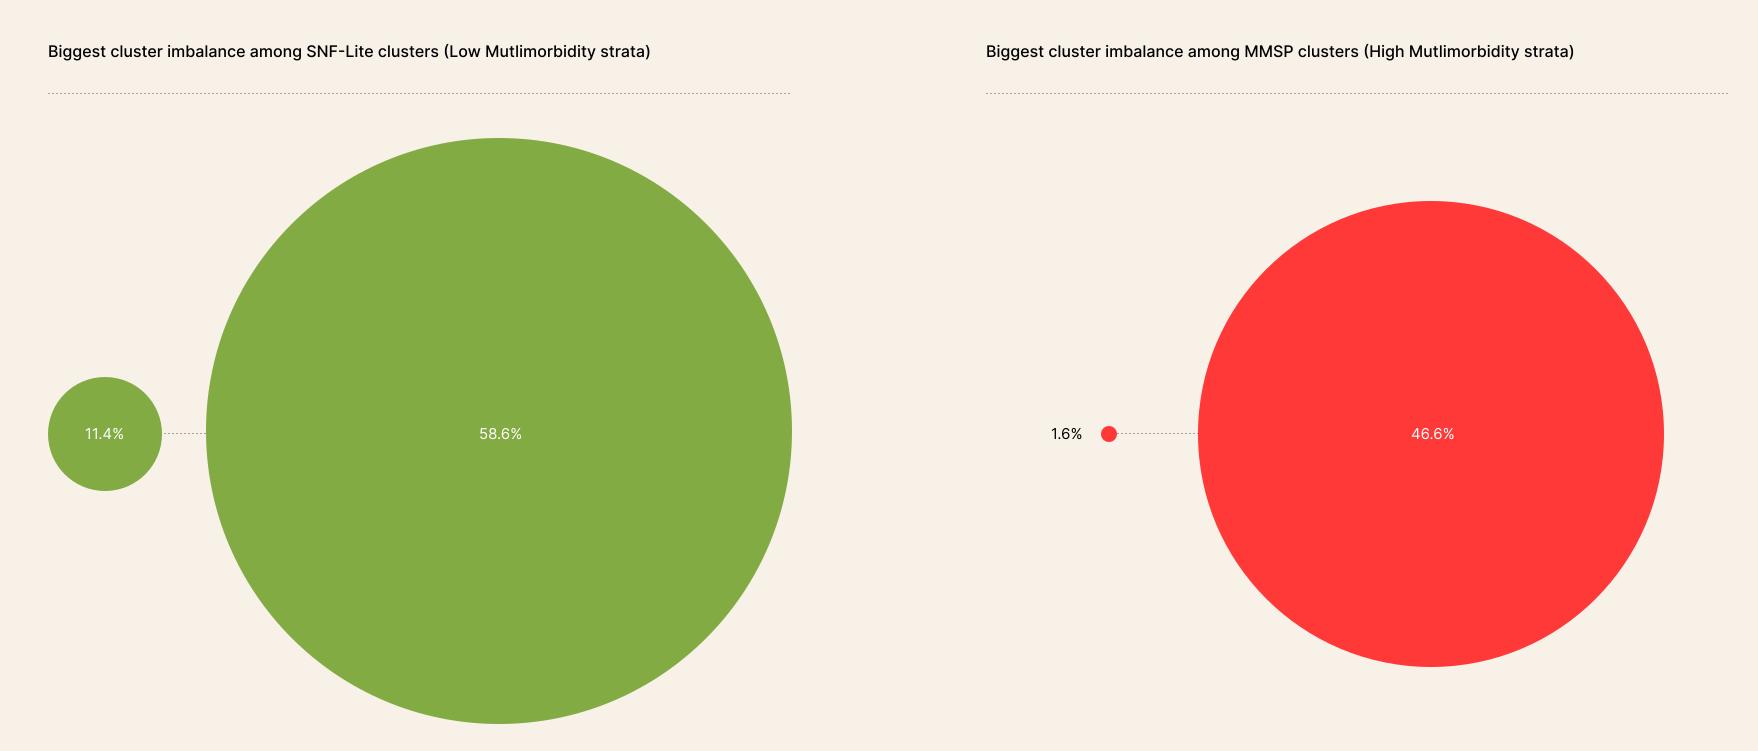
\includegraphics[width=0.8\linewidth]{../PortfolioMain/Cluster Sizes} 

}

\caption[Cluster balance in SNF-lite versus MMSP phenotypes]{Cluster balance in SNF-lite versus MMSP phenotypes. Each bubble represents the smallest and largest clusters in the most imbalanced stratum for each method.}\label{fig:cluster_sizes}
\end{figure}

\subsection{\texorpdfstring{\textbf{Concordance \&
Complementarity}}{Concordance \& Complementarity}}\label{concordance-complementarity}

We next compared MMSP and SNF-lite labelings within each multimorbidity
stratum. Cross-tabulations and pairwise Venn diagrams showed that no
SNF-lite cluster mapped cleanly onto a single MMSP cluster or vice
versa; most clusters shared only partial overlap.

Agreement between MMSP and SNF-lite labels was quantified within each
multimorbidity stratum using Adjusted Rand Index (ARI) and Normalised
Mutual Information (NMI). Values near 0 indicate little more than random
overlap; values near 1 indicate near-identical partitions.

\begin{longtable}[]{@{}
  >{\raggedright\arraybackslash}p{(\linewidth - 12\tabcolsep) * \real{0.1212}}
  >{\centering\arraybackslash}p{(\linewidth - 12\tabcolsep) * \real{0.1515}}
  >{\centering\arraybackslash}p{(\linewidth - 12\tabcolsep) * \real{0.1515}}
  >{\centering\arraybackslash}p{(\linewidth - 12\tabcolsep) * \real{0.1515}}
  >{\centering\arraybackslash}p{(\linewidth - 12\tabcolsep) * \real{0.1515}}
  >{\centering\arraybackslash}p{(\linewidth - 12\tabcolsep) * \real{0.1515}}
  >{\raggedright\arraybackslash}p{(\linewidth - 12\tabcolsep) * \real{0.1212}}@{}}
\toprule\noalign{}
\begin{minipage}[b]{\linewidth}\raggedright
Stratum
\end{minipage} & \begin{minipage}[b]{\linewidth}\centering
Sample size (N)
\end{minipage} & \begin{minipage}[b]{\linewidth}\centering
\(K_{MMSP}\)
\end{minipage} & \begin{minipage}[b]{\linewidth}\centering
\(K_{SNF}\)
\end{minipage} & \begin{minipage}[b]{\linewidth}\centering
ARI
\end{minipage} & \begin{minipage}[b]{\linewidth}\centering
NMI
\end{minipage} & \begin{minipage}[b]{\linewidth}\raggedright
Concordance summary
\end{minipage} \\
\midrule\noalign{}
\endhead
\bottomrule\noalign{}
\endlastfoot
Low MM & 4,183 & 4 & 3 & 0.078 & 0.119 & Low concordance; large SNF
clusters mix several MMSP phenotypes. \\
Mid MM & 3,822 & 3 & 3 & 0.141 & 0.152 & Highest overlap, but still
partial nesting and many-to-many mapping. \\
High MM & 1,100 & 5 & 3 & 0.098 & 0.129 & Low concordance; each SNF
cluster draws from multiple MMSP clusters. \\
\end{longtable}

\marginnote{Table: Concordance between MMSP and SNF-lite phenotypes. ARI and NMI values around 0.1 indicate that MMSP and SNF-lite capture related but distinct structure; neither solution is a simple relabelling of the other.}

Concordance metrics were modest (\textbf{ARI 0.08--0.14; NMI
0.12--0.15}), indicating that the two methods capture related but
distinct structure in the patient space. Together with the
cross-validated prognostic analysis---where both labelings improved
discrimination over a clinical base model but SNF-lite yielded the
largest \(\Delta\)C---this suggests that MMSP and SNF-lite provide
\textbf{complementary phenotypic views} rather than redundant
partitions. We therefore treat SNF-lite phenotypes as the primary
clustering solution, with MMSP phenotypes providing a physiology-focused
sensitivity and interpretability check within comorbidity strata.

\begin{figure}

{\centering \includegraphics[width=0.32\linewidth]{../reports/figures/sankey_Low_MM} \includegraphics[width=0.32\linewidth]{../reports/figures/sankey_Mid_MM} \includegraphics[width=0.32\linewidth]{../reports/figures/sankey_High_MM} 

}

\caption[Sankey diagrams showing patient flow between MMSP and SNF clusters in Low (left), Mid (center), and High (right) multimorbidity strata]{Sankey diagrams showing patient flow between MMSP and SNF clusters in Low (left), Mid (center), and High (right) multimorbidity strata.}\label{fig:sankeys}
\end{figure}

\subsection{High multimorbidity
stratum}\label{high-multimorbidity-stratum}

In the high multimorbidity stratum, SNF-lite identified three large
clusters that differed both in chronic disease burden and in acute
physiological derangement. The first cluster was dominated by patients
with acute renal failure or multi-organ system failure on a background
of substantial multimorbidity. This group had the highest concentration
of organ-failure diagnoses, frequent diabetes and malignancy, and the
most abnormal acute physiology scores (higher APS/SPS/AVTISS) compared
with the other high-multimorbidity clusters. Together, these features
are consistent with a ``diabetic multi-organ failure'' profile
representing the most acutely unwell segment of the high-burden cohort.

The second high-multimorbidity cluster was characterised by a
predominance of chronic cardio-pulmonary and hepatic disease. Congestive
heart failure and COPD were much more common here than in the other
clusters, and cirrhosis was also enriched, whereas multi-organ failure
codes were less frequent. Acute physiology scores in this cluster were
closer to or slightly better than the stratum average, and oxygenation
and albumin levels were relatively preserved. Clinically, this group
resembles a chronic ``cardio-pulmonary plus liver disease'' phenotype:
patients with substantial chronic disease burden but without the same
degree of acute decompensation seen in the organ-failure cluster.

The third high-multimorbidity cluster was defined by very high
prevalence of congestive heart failure and diabetes, together with a
high burden of solid tumours, including lung cancer, but comparatively
little recorded multi-organ failure. Patients in this cluster had the
least severe acute physiology among the high-multimorbidity groups, with
better oxygenation and less marked derangement in renal and biochemical
markers. This pattern is most consistent with a ``chronic
cardiometabolic plus cancer'' phenotype: individuals with extensive
chronic illness, particularly heart failure and malignancy, but without
the extreme acute instability of the multi-organ failure cluster.

\subsection{Mid multimorbidity
stratum}\label{mid-multimorbidity-stratum}

Within the intermediate multimorbidity stratum, the three clusters also
separated into recognisable clinical profiles. One cluster was dominated
by chronic respiratory disease: COPD prevalence was markedly higher than
in the rest of the cohort, with accompanying but more modest levels of
heart failure, cancer and other comorbidities. Patients in this group
were older on average, with only mildly abnormal acute physiology and
modest impairment of oxygenation, suggesting an ``older COPD-dominant
chronic respiratory'' phenotype rather than fulminant respiratory
failure.

A second cluster in the mid-multimorbidity stratum was defined by high
rates of acute renal failure and multi-organ system failure, often in
combination with malignancy and cirrhosis. Coma was also more common in
this group. These patients tended to be somewhat younger than the
COPD-dominant cluster but had substantially worse acute physiology
scores, lower albumin and more deranged biochemical markers, indicating
a ``younger high-acuity multi-organ failure with malignancy and liver
disease'' phenotype.

The third mid-multimorbidity cluster was characterised by high
prevalence of heart failure and an exceptionally high burden of solid
tumours, particularly lung and colorectal cancers, but relatively low
rates of explicit multi-organ failure. Despite this heavy oncological
and cardiac comorbidity, acute physiology scores, oxygenation and renal
indices were the most favourable among the mid-multimorbidity clusters.
This pattern is consistent with a ``compensated heart failure plus solid
tumour'' phenotype: patients with substantial chronic disease,
especially cancer, who remain comparatively stable at the time of
admission.

\subsection{Low multimorbidity
stratum}\label{low-multimorbidity-stratum}

In the low multimorbidity stratum, where patients by definition had
fewer recorded chronic conditions, SNF-lite still identified three
clinically coherent clusters. One cluster comprised patients with a very
high burden of solid tumours---particularly lung and colon cancer---but
relatively low levels of other comorbidities. Acute physiology in this
group was comparatively preserved, with good oxygenation, reasonable
renal function and less extreme derangement of vital signs. This pattern
represents a ``low-acuity solid tumour'' phenotype: oncology-dominant
patients with limited additional multimorbidity.

A second cluster in the low-multimorbidity stratum was strongly
characterised by coma. Coma diagnoses were frequent, whereas other
chronic comorbidities were less prominent, and organ-failure codes were
only moderately elevated. Physiological markers suggested significant
neurological compromise with only modest systemic derangement compared
with the multi-organ failure clusters. This cluster can be viewed as a
``neurologic catastrophe/coma'' phenotype within an otherwise less
multimorbid population.

The third low-multimorbidity cluster was distinguished by very high
prevalence of acute renal failure or multi-organ system failure, often
in patients with relatively few chronic diagnoses. Acute physiology
scores were clearly worse than in the other low-multimorbidity clusters,
with more impaired oxygenation and less favourable biochemical profiles.
This group represents an ``acute multi-organ failure in otherwise
low-comorbidity patients'' phenotype, capturing individuals who are
severely unwell at presentation despite limited baseline multimorbidity.

Taken together, these nine clusters map onto intuitive clinical patterns
spanning chronic cardio-pulmonary disease, malignancy-dominant states,
neurological catastrophe and acute multi-organ failure, with each
multimorbidity stratum showing its own spectrum of acute severity and
disease composition.

Cluster solutions from the SNF-lite models yielded three clinically
distinct profiles within each multimorbidity stratum. Below we describe
the composition and acute physiology of these clusters, using the
cohort-level characteristics (high mortality, high prevalence of
multi-organ failure and malignancy) as the reference context.

\marginnote{Table X. Qualitative clinical profiles of SNF-lite clusters within each multimorbidity stratum.}

\begin{longtable}[]{@{}
  >{\raggedright\arraybackslash}p{(\linewidth - 8\tabcolsep) * \real{0.0491}}
  >{\raggedright\arraybackslash}p{(\linewidth - 8\tabcolsep) * \real{0.0402}}
  >{\raggedright\arraybackslash}p{(\linewidth - 8\tabcolsep) * \real{0.2411}}
  >{\raggedright\arraybackslash}p{(\linewidth - 8\tabcolsep) * \real{0.3214}}
  >{\raggedright\arraybackslash}p{(\linewidth - 8\tabcolsep) * \real{0.3482}}@{}}
\toprule\noalign{}
\begin{minipage}[b]{\linewidth}\raggedright
Stratum
\end{minipage} & \begin{minipage}[b]{\linewidth}\raggedright
Cluster
\end{minipage} & \begin{minipage}[b]{\linewidth}\raggedright
Phenotype label
\end{minipage} & \begin{minipage}[b]{\linewidth}\raggedright
Dominant comorbidities / features
\end{minipage} & \begin{minipage}[b]{\linewidth}\raggedright
Acute physiology profile (relative within stratum)
\end{minipage} \\
\midrule\noalign{}
\endhead
\bottomrule\noalign{}
\endlastfoot
High MM & H1 & Diabetic multi-organ failure & High burden of acute renal
failure / multi-organ system failure, frequent diabetes and cancer, some
dementia & Most acutely unwell; highest acute physiology scores,
impaired oxygenation, biochemical derangement \\
High MM & H2 & Cardio-pulmonary plus liver disease & Enriched for
chronic heart failure, COPD and cirrhosis; moderate diabetes and cancer
& Intermediate severity; acute physiology close to stratum average,
oxygenation and albumin relatively preserved \\
High MM & H3 & Cardiometabolic plus solid tumours & Very high prevalence
of heart failure and diabetes with substantial solid tumour burden
(e.g.~lung, other) & Least acutely deranged; relatively preserved
oxygenation and renal function despite heavy chronic disease \\
Mid MM & M1 & Older COPD-dominant chronic respiratory & Marked excess of
COPD with coexisting but moderate heart failure, diabetes and cancer &
Older patients; mild-to-moderate acute derangement, modest impairment of
oxygenation \\
Mid MM & M2 & Multi-organ failure with malignancy and cirrhosis & High
rates of acute renal failure / multi-organ failure, malignancy
(including metastatic) and cirrhosis; more coma & Younger-to-midlife
profile; most abnormal acute physiology, low albumin and more deranged
biochemical markers \\
Mid MM & M3 & Compensated heart failure plus solid tumours & High
prevalence of heart failure and solid tumours (lung, colorectal),
relatively few explicit organ-failure codes & Best preserved acute
physiology in this stratum; near-normal oxygenation, renal indices and
vital signs \\
Low MM & L1 & Low-acuity solid tumour & Dominated by solid tumours
(especially lung and colon cancer) with few additional chronic
conditions & Lowest acute severity; good oxygenation and renal function,
limited physiological derangement \\
Low MM & L2 & Neurologic catastrophe / coma & Very high frequency of
coma diagnoses; relatively low chronic multimorbidity and modest
organ-failure burden & Marked neurological compromise with only moderate
systemic physiological derangement \\
Low MM & L3 & Acute multi-organ failure with low baseline multimorbidity
& Very high prevalence of acute renal failure / multi-organ failure in
patients with few recorded chronic diseases & Most acutely unwell in
this stratum; impaired oxygenation and worse biochemical profiles
despite low multimorbidity \\
\end{longtable}

\emph{Kruskal-Wallis Ranking (Best Discriminators First)}

\begin{longtable}[]{@{}llrrrrlr@{}}
\toprule\noalign{}
Variable & .y. & n & statistic & df & p & method & p.adj \\
\midrule\noalign{}
\endhead
\bottomrule\noalign{}
\endlastfoot
aps & Value & 9105 & 2971.76456 & 8 & 0 & Kruskal-Wallis & 0 \\
alb & Value & 9105 & 621.56034 & 8 & 0 & Kruskal-Wallis & 0 \\
pafi & Value & 9105 & 578.97075 & 8 & 0 & Kruskal-Wallis & 0 \\
age & Value & 9105 & 564.44932 & 8 & 0 & Kruskal-Wallis & 0 \\
temp & Value & 9105 & 328.86150 & 8 & 0 & Kruskal-Wallis & 0 \\
wblc & Value & 9105 & 257.48257 & 8 & 0 & Kruskal-Wallis & 0 \\
hrt & Value & 9105 & 235.20340 & 8 & 0 & Kruskal-Wallis & 0 \\
crea & Value & 9105 & 228.16551 & 8 & 0 & Kruskal-Wallis & 0 \\
meanbp & Value & 9105 & 93.60548 & 8 & 0 & Kruskal-Wallis & 0 \\
\end{longtable}

\emph{Physiological Profiles}

\begin{figure*}
\includegraphics{Manuscript_files/figure-latex/fig-profiles-1} \caption[Figure 2]{Figure 2: Physiological and Comorbidity Profiles. Standardized median values (Z-scores) for key discriminators across the three clusters within each multimorbidity stratum.}\label{fig:fig-profiles}
\end{figure*}

\subsection{\texorpdfstring{\textbf{Outcome
associations}}{Outcome associations}}\label{outcome-associations}

\subsection{Primary outcome associations (365-day
mortality)}\label{cox-primary}

Within each multimorbidity stratum, I estimated adjusted associations
between SNF-lite phenotype membership and 365-day all-cause mortality
using Cox proportional hazards models, with cluster as the exposure and
adjustment for age (standardised), sex, multimorbidity count
(standardised), and acute physiology severity (APS, standardised).
Cluster membership remained independently prognostic after adjustment.
In the high multimorbidity cohort (N=1100), both High\_MM\_1 and
High\_MM\_2 had lower mortality hazards than the reference High\_MM\_0
(High\_MM\_1 vs High\_MM\_0: HR 0.57 {[}0.39--0.82{]}; High\_MM\_2 vs
High\_MM\_0: HR 0.51 {[}0.37--0.70{]}). In the mid stratum (N=3822),
Mid\_MM\_1 showed the highest adjusted risk relative to Mid\_MM\_0 (HR
1.87 {[}1.56--2.23{]}), with a smaller but still significant elevation
for Mid\_MM\_2 (HR 1.30 {[}1.11--1.53{]}). In the low stratum (N=4183),
the coma-dominant phenotype Low\_MM\_1 had markedly higher adjusted risk
than Low\_MM\_0 (HR 2.36 {[}1.93--2.89{]}), while Low\_MM\_2 had lower
adjusted hazard than Low\_MM\_0 (HR 0.59 {[}0.49--0.73{]}), consistent
with long-term risk being driven by underlying disease composition in
addition to acute severity. APS was the strongest and most consistent
covariate across strata (HR \textasciitilde1.4--1.6 per 1 SD increase).

Proportional hazards diagnostics based on Schoenfeld residuals indicated
departures from strict PH assumptions even after truncation to 365 days;
hazard ratios are therefore interpreted as average effects over the
1-year horizon and are presented alongside unadjusted KM curves as
supporting evidence.

In addition to the adjusted Cox models reported above, I ran supporting
outcome analyses to contextualise these findings, including unadjusted
Kaplan--Meier curves with logrank tests, and non-parametric comparisons
of ICU length of stay and total medical costs across phenotypes. These
supplementary outputs are provided in the Supplementary section (figures
and tables), alongside cluster profile summaries used for phenotype
interpretation.

\subsubsection{High multimorbidity
stratum}\label{high-multimorbidity-stratum-1}

Reference phenotype: \textbf{High\_MM\_0}.

\begin{longtable}[]{@{}lrr@{}}
\toprule\noalign{}
Term & Adjusted HR (95\% CI) & p-value \\
\midrule\noalign{}
\endhead
\bottomrule\noalign{}
\endlastfoot
High\_MM\_1 vs High\_MM\_0 & 0.57 (0.39--0.82) & 0.003 \\
High\_MM\_2 vs High\_MM\_0 & 0.51 (0.37--0.70) & 2.0e-05 \\
Age (per 1 SD) & 0.96 (0.82--1.11) & 0.576 \\
Male (vs female) & 1.24 (1.03--1.50) & 0.025 \\
Multimorbidity count (per 1 SD) & 1.02 (0.88--1.18) & 0.798 \\
Acute physiology (APS, per 1 SD) & 1.43 (1.20--1.70) & 4.0e-05 \\
\end{longtable}

\begin{figure}
\centering
\pandocbounded{\includegraphics[keepaspectratio]{/Users/harisreedeth/Desktop/D/personal/ProjectMAIP/PrimaryOutcomesCodebook/TechnicalDocumentation_files/figure-html/KM_curves-1.png}}
\caption{Fig A. Adjusted hazard ratios for High multimorbidity stratum.}
\end{figure}

\begin{center}\rule{0.5\linewidth}{0.5pt}\end{center}

\subsubsection{Mid multimorbidity
stratum}\label{mid-multimorbidity-stratum-1}

Reference phenotype: \textbf{Mid\_MM\_0}.

\begin{longtable}[]{@{}lrr@{}}
\toprule\noalign{}
Term & Adjusted HR (95\% CI) & p-value \\
\midrule\noalign{}
\endhead
\bottomrule\noalign{}
\endlastfoot
Mid\_MM\_1 vs Mid\_MM\_0 & 1.87 (1.56--2.23) & 2.1e-11 \\
Mid\_MM\_2 vs Mid\_MM\_0 & 1.30 (1.11--1.53) & 0.002 \\
Age (per 1 SD) & 1.28 (1.17--1.40) & 1.1e-07 \\
Male (vs female) & 1.06 (0.96--1.17) & 0.239 \\
Multimorbidity count (per 1 SD) & 0.92 (0.83--1.01) & 0.101 \\
Acute physiology (APS, per 1 SD) & 1.63 (1.49--1.78) & 2.6e-26 \\
\end{longtable}

\begin{figure}
\centering
\pandocbounded{\includegraphics[keepaspectratio]{/Users/harisreedeth/Desktop/D/personal/ProjectMAIP/PrimaryOutcomesCodebook/TechnicalDocumentation_files/figure-html/KM_curves-2.png}}
\caption{Fig B. Adjusted hazard ratios for Mid multimorbidity stratum.}
\end{figure}

\begin{center}\rule{0.5\linewidth}{0.5pt}\end{center}

\subsubsection{Low multimorbidity
stratum}\label{low-multimorbidity-stratum-1}

Reference phenotype: \textbf{Low\_MM\_0}.

\begin{longtable}[]{@{}lrr@{}}
\toprule\noalign{}
Term & Adjusted HR (95\% CI) & p-value \\
\midrule\noalign{}
\endhead
\bottomrule\noalign{}
\endlastfoot
Low\_MM\_1 vs Low\_MM\_0 & 2.36 (1.93--2.89) & 1.2e-15 \\
Low\_MM\_2 vs Low\_MM\_0 & 0.59 (0.49--0.73) & 1.5e-04 \\
Age (per 1 SD) & 1.22 (1.11--1.34) & 5.3e-05 \\
Male (vs female) & 1.06 (0.93--1.21) & 0.427 \\
Multimorbidity count (per 1 SD) & 1.66 (1.47--1.87) & 9.9e-17 \\
Acute physiology (APS, per 1 SD) & 1.48 (1.33--1.65) & 2.2e-11 \\
\end{longtable}

\begin{figure}
\centering
\pandocbounded{\includegraphics[keepaspectratio]{/Users/harisreedeth/Desktop/D/personal/ProjectMAIP/PrimaryOutcomesCodebook/TechnicalDocumentation_files/figure-html/KM_curves-3.png}}
\caption{Fig C. Adjusted hazard ratios for Low multimorbidity stratum.}
\end{figure}

\subsection{\texorpdfstring{\textbf{Surrogate trees and LLM-derived
rulecards}}{Surrogate trees and LLM-derived rulecards}}\label{surrogate-trees-and-llm-derived-rulecards}

\subsection{Surrogate decision trees for explainable
phenotypes}\label{surrogate-decision-trees-for-explainable-phenotypes}

For each stratum of multimorbidity (High\_MM, Mid\_MM, Low\_MM), we
trained a separate decision tree classifier to approximate the
SNF-derived phenotypes. The input features were the same harmonised
baseline variables used in the clustering stage, and the outcome was the
stratum-specific phenotype label (e.g.~High\_MM\_0--2). Trees were grown
with depth and leaf-size constraints to avoid overfitting (maximum depth
and minimum samples per leaf tuned by grid search with
cross-validation), and class weights were balanced to account for modest
differences in phenotype prevalence. Hyperparameter selection was based
on macro-averaged F1 and overall accuracy, averaged across repeated
cross-validation; the chosen settings and per-stratum performance are
reported in Supplementary Table Sx. The final fitted trees were then
used as ``surrogate'' models from which we extracted all decision paths
terminating in each phenotype. Each unique leaf path corresponds to one
JSON-encoded rule of the form ``feature--operator--threshold'' together
with its observed support and purity.

\subsection{Retrieval-augmented corpus for rule
translation}\label{retrieval-augmented-corpus-for-rule-translation}

To translate these machine-readable rules into clinician-facing
descriptions, we built a small, frozen knowledge base and used it within
a retrieval-augmented generation (RAG) pattern. The corpus comprised
three components: (i) a variable dictionary
(\texttt{variable\_dictionary.json}) containing, for each feature, a
short display name, a plain-language description, units, a typical range
and (where applicable) the expected direction of risk; (ii) one
phenotype summary per label
(\texttt{Phenotype\ \textless{}stratum\_label\textgreater{}.md}),
providing a concise, data-driven description of its comorbidity
composition, acute physiology profile and survival tendencies; and (iii)
a style guide (\texttt{style\_guide.md}) specifying how narratives,
rulecards and ASCII flowcharts should be phrased. The corpus was treated
as immutable (``frozen'') before LLM generation to ensure
reproducibility.

For each phenotype, a translation script assembled a compact prompt by
combining four elements: (i) the JSON rule paths for that phenotype,
(ii) the corresponding phenotype summary, (iii) the subset of
variable-dictionary entries for the features appearing in those rules,
and (iv) an excerpt of the style guide. In conceptual terms, this
corresponds to a small vector index over markdown/JSON documents where
the phenotype label and feature names define the query; in practice, we
explicitly selected the relevant snippets based on the rule paths, so
that only phenotype-specific material was injected into the context.

\subsection{LLM configuration and deterministic
instructions}\label{llm-configuration-and-deterministic-instructions}

Rule translation was performed with a remote, general-purpose chat model
(GPT-4.1-mini, 8k context, accessed via API). The model was instructed
via a fixed system prompt to behave as a deterministic translator rather
than a diagnostic agent. Specifically, it was told to: (i) preserve
every logical element of the JSON rules (feature, operator, numeric
threshold) in an equivalent IF/THEN form; (ii) avoid introducing any new
variables, cut-points or phenotypes; (iii) refrain from treatment or
management advice; and (iv) always emit exactly three sections, with
fixed headings:

\begin{Shaded}
\begin{Highlighting}[]
\AttributeTok{* \textasciigrave{}Phenotype \textless{}label\textgreater{} – \textless{}short title\textgreater{}\textasciigrave{}}
\AttributeTok{* \textasciigrave{}Key idea:\textasciigrave{} – one or two sentences summarising the typical patient}
\AttributeTok{* \textasciigrave{}Rulecard:\textasciigrave{} – a bullet list of explicit IF/THEN rules}
\AttributeTok{* \textasciigrave{}ASCII flowchart:\textasciigrave{} – a simple text flowchart mirroring the same branches.}
\end{Highlighting}
\end{Shaded}

The prompts also explicitly forbade regurgitating the JSON or the
style-guide text itself. Generation used a low temperature (0--0.1) and
a sufficiently high token budget to avoid truncation, so that outputs
were essentially deterministic given the fixed inputs.

For each of the nine phenotypes (three per stratum), the pipeline
produced a canonical markdown rulecard
(\texttt{rulecard\_\textless{}label\textgreater{}.md}) containing a
short narrative (``Key idea''), a human-readable rulecard and an ASCII
flowchart skeleton representing the same decision paths. The entire
process was wrapped in a single command-line entry point
(\texttt{python\ -m\ src.cli\ build-rulecards\ …}), which (i)
regenerates the surrogate ruleset if needed, (ii) rebuilds the prompts
from the frozen corpus, (iii) calls the remote LLM, and (iv) runs the
validation checks described below.

\subsection{Programmatic quality control of
rulecards}\label{programmatic-quality-control-of-rulecards}

We implemented a dedicated validation script to check fidelity between
the JSON rules, the variable dictionary and the LLM-generated texts.
First, for each stratum we loaded the canonical
\texttt{rule\_ruleset.json} and the corresponding rulecards. All
decision paths associated with a given phenotype were counted (JSON rule
count), and the rulecard text was parsed line-by-line to identify bullet
points beginning with ``- IF''. For each JSON condition, we required
that (i) the canonical feature name appeared in at least one ``- IF''
line, and (ii) a string representation of the threshold (with several
numeric formats) appeared in the same line. Any missing
feature--threshold pairing flagged that phenotype as having incomplete
coverage. We summarised these checks in per-stratum CSV files recording,
for each phenotype, the number of JSON rules, number of textual IF rules
and flags for missing features or mismatched thresholds.

Second, we assessed dictionary alignment. For every feature used in the
surrogate rules, we confirmed that an entry existed in the variable
dictionary and that the canonical feature name appeared somewhere in the
corresponding rulecard. We also recorded whether the name appeared in
parentheses or code formatting (e.g.~``acute physiology score (aps)''),
as a proxy for readability. These checks were again summarised in
per-stratum CSV tables.

Finally, we optionally verified that the synthetic logic of the JSON
rules was consistent with the fitted surrogate tree. For each leaf path,
we constructed a synthetic feature vector that lay inside the
corresponding decision region (by choosing values slightly within each
inequality) and passed it through the trained tree. The predicted label
was compared with the phenotype label attached to that path; mismatches
were recorded for manual inspection. This step provides a sanity check
that the exported rule paths correctly reflect the behaviour of the
surrogate classifier.

\subsection{\texorpdfstring{\textbf{Surrogate fidelity and rulecard
generation}}{Surrogate fidelity and rulecard generation}}\label{surrogate-fidelity-and-rulecard-generation}

\subsection{Surrogate tree
performance}\label{surrogate-tree-performance}

\marginnote{Table X. Cross-validated fidelity of decision tree surrogates to SNF phenotypes, by multimorbidity stratum.}

\begin{longtable}[]{@{}lll@{}}
\toprule\noalign{}
Stratum & CV accuracy (mean ± SD) & Macro--F1 (mean ± SD) \\
\midrule\noalign{}
\endhead
\bottomrule\noalign{}
\endlastfoot
High MM & 0.741 ± 0.027 & 0.744 ± 0.026 \\
Mid MM & 0.821 ± 0.004 & 0.797 ± 0.007 \\
Low MM & 0.900 ± 0.007 & 0.877 ± 0.013 \\
\end{longtable}

The surrogate trees provided a compact, reasonably faithful
approximation to the SNF-derived phenotypes. Cross-validated performance
was strongest in the low-multimorbidity stratum and lowest in the
high-multimorbidity stratum, consistent with the greater clinical
heterogeneity of the latter. Macro-averaged F1 and overall accuracy by
stratum are reported in Table X. Briefly, all three surrogates achieved
moderate-to-high macro-F1, indicating that no single phenotype dominated
the fit, and inspection of the trees confirmed that they were small
enough to be interpretable while capturing the main decision structure
of the underlying clusters.

\begin{figure*}
\includegraphics[width=33.33in]{../reports/figures/cf_all_strata} \caption[Figure ]{Figure : Confusion Matrices from surrogate models used in SNF clusters}\label{fig:ConfMatrices}
\end{figure*}

Across strata, the fitted trees yielded between one and seven terminal
rules per phenotype (median ≈4), each corresponding to a distinct
combination of comorbidity groups and acute physiology cut-points.
Cancer-dominated phenotypes in the low-multimorbidity stratum were
typically represented by a single, simple rule, whereas multi-organ
failure phenotypes in the high- and mid-multimorbidity strata required
several leaf paths to cover different ranges of physiology and support
intensity.

\subsection{Fidelity of LLM-generated
rulecards}\label{fidelity-of-llm-generated-rulecards}

The RAG-based translation pipeline successfully produced narrative
descriptions, rulecards and ASCII flowcharts for all nine phenotypes.
Programmatic checks confirmed that every JSON rule was represented in
the corresponding textual rulecard: for each phenotype, the number of
``- IF'' rules in the markdown was at least as large as the number of
leaf paths in the surrogate tree, and all feature--threshold pairs
extracted from the JSON were detected in the same lines of the rulecard.
No missing features or mismatched thresholds were identified in the
final canonical rulecards after minor manual edits to enforce one IF
condition per line.

Dictionary alignment was also complete: every feature appearing in any
surrogate rule had a corresponding entry in the variable dictionary and
was mentioned by its canonical name in the rulecard text. Many features
were additionally referenced in parentheses after a plain-language
description (for example, ``Acute Physiology Score (aps)'' or
``Do-Not-Resuscitate status: no DNR order (dnr\_no\_dnr)''), which helps
bridge model-centric and clinician-centric terminology.

In the optional synthetic-profile verification, we generated 38
synthetic patient profiles spanning all decision paths (14 in the high-,
13 in the mid- and 11 in the low-multimorbidity strata). For every
profile, the surrogate tree's prediction matched the phenotype label
attached to the corresponding rule path, yielding 100\% agreement across
strata. This suggests that the exported JSON rules faithfully captured
the behaviour of the fitted surrogate models, and that the
LLM-translated rulecards, which were constrained to mirror those JSON
rules, provide a logically faithful narrative representation of the
phenotypes.

Complete rulecards and ASCII flowcharts for all nine phenotypes are
provided in the Supplementary Material, together with the surrogate-tree
hyperparameters, cross-validation metrics and programmatic QC summaries.

\section{\texorpdfstring{\textbf{Supplementary
analyses}}{Supplementary analyses}}\label{supplementary-analyses}

Across all three multimorbidity strata, the SNF-lite phenotypes show
clear separation in 365-day survival, indicating that the clusters
capture clinically meaningful risk heterogeneity \emph{within} baseline
multimorbidity burden. In the High\_MM stratum, High\_MM\_0 exhibits
markedly worse early survival than the other two clusters, while
High\_MM\_2 shows the most favourable survival trajectory over the first
year (High\_MM\_1 is intermediate). In the Mid\_MM stratum, Mid\_MM\_1
separates as the highest-risk cluster with steep early mortality,
whereas Mid\_MM\_0 and Mid\_MM\_2 remain substantially higher and closer
together. In the Low\_MM stratum, Low\_MM\_1 is clearly the highest-risk
cluster, while Low\_MM\_0 and Low\_MM\_2 show materially better 365-day
survival with only modest late divergence.

\begin{figure*}
\includegraphics[width=46.67in]{../reports/outcomes_supporting_365d/figures/km_all_strata} \caption[Figure]{Figure: 365-day Kaplan–Meier curves by SNF-lite phenotype (stratified by multimorbidity burden)}\label{fig:KM_curves}
\end{figure*}

Consistent with the survival separation, length of stay (LOS) and total
cost also differ significantly by cluster within each stratum
(Kruskal--Wallis). These differences support the interpretation that the
phenotypes are not only clinically coherent (composition/physiology) but
also prognostically and resource-relevant. These KM/LOS/cost results are
the supporting descriptive layer; the primary inference should be
reported using the adjusted, stratum-specific Cox models in R
(age/sex/multimorbidity count/severity adjustment), with the KM plots
presented as an intuitive visual confirmation of risk ordering.

\subsubsection{Table: Global differences in outcomes by stratum
(supporting
analyses)}\label{table-global-differences-in-outcomes-by-stratum-supporting-analyses}

\marginnote{Table: Global differences in outcomes by stratum (supporting analyses)}

\begin{longtable}[]{@{}
  >{\raggedright\arraybackslash}p{(\linewidth - 8\tabcolsep) * \real{0.0909}}
  >{\raggedleft\arraybackslash}p{(\linewidth - 8\tabcolsep) * \real{0.0519}}
  >{\raggedleft\arraybackslash}p{(\linewidth - 8\tabcolsep) * \real{0.3247}}
  >{\raggedleft\arraybackslash}p{(\linewidth - 8\tabcolsep) * \real{0.2597}}
  >{\raggedleft\arraybackslash}p{(\linewidth - 8\tabcolsep) * \real{0.2727}}@{}}
\toprule\noalign{}
\begin{minipage}[b]{\linewidth}\raggedright
Stratum
\end{minipage} & \begin{minipage}[b]{\linewidth}\raggedleft
N
\end{minipage} & \begin{minipage}[b]{\linewidth}\raggedleft
Overall log-rank p (365d)
\end{minipage} & \begin{minipage}[b]{\linewidth}\raggedleft
LOS Kruskal--Wallis p
\end{minipage} & \begin{minipage}[b]{\linewidth}\raggedleft
Cost Kruskal--Wallis p
\end{minipage} \\
\midrule\noalign{}
\endhead
\bottomrule\noalign{}
\endlastfoot
High\_MM & 1100 & 1.5e-35 & 1.3e-17 & 1.3e-50 \\
Mid\_MM & 3822 & 8.9e-71 & 8.0e-76 & 1.0e-146 \\
Low\_MM & 4183 & 2.8e-95 & 2.2e-157 & 1.5e-157 \\
\end{longtable}

Although effect-size estimates (medians and interquartile ranges) are
reported separately, these p-values confirm that the phenotypes map onto
distinct patterns of healthcare utilisation: clusters with more acute
physiological derangement and multi-organ failure tend to have longer
stays and higher costs, while the low-acuity phenotypes have
substantially shorter stays and lower expenditure.

\textbf{Taken together, these results show that the clustered phenotypes
are not merely proxies for APS or comorbidity count: cluster membership
remains strongly associated with mortality after adjusting for acute
physiology within each comorbidity stratum.}

\bibliography{skeleton.bib}



\end{document}
